%% The following is a directive for TeXShop to indicate the main file
%!TEX root = ../diss.tex

\chapter[MRI and histology of vascular function in xenografts using \acs{HPG-GdF}]{Multi-modal magnetic resonance imaging and histology of vascular function in xenografts using macromolecular contrast agent hyperbranched polyglycerol (HPG-GdF)}
\label{ch:HPG}

\section{Introduction}
The vascular network in tumour tissue is abnormal, often resulting in vessels that have variable flow rates and high permeability relative to blood vessels in normal tissue~\cite{McDonald:2002ut}.
Dynamic contrast-enhanced magnetic resonance imaging (DCE-MRI) is a useful tool for non-invasively assessing tumour vasculature by imaging and measuring concentrations of \acs{CA} delivered to tumours by the vessels~\cite{OConnor:2012ie,Barrett:2006jx,Leach:2003fy}.
The appeal of a dynamic, non-invasive approach for measuring tumour vascular function in the clinic is clear.
Such data is applicable in the field of assessing treatment response for vascular targeting therapies~\cite{OConnor:2012ie,Barrett:2006jx,Leach:2003fy}.
In addition to utility as a treatment biomarker, vascular function data may be able to predict which tumours are likely to respond to therapy~\cite{DeBruyne:2012cq,Kelly:2011cf,Bains:2009hh}, or which regions or tumours have greater heterogeneity in their microenvironment~\cite{OConnor:2011jm,Alic:2011hw}.
The issue of its limited access for anticancer drugs in solid tumours is significant~\cite{Minchinton:2006gs}, particularly given the efforts to create nanoparticle therapeutics that target the tumour via the \acs{EPR} effect~\cite{Jain:2001uf,Iyer:2006gf,Chauhan:2011fi}.
A translatable imaging protocol and suitable contrast agent that yields meaningful and reproducible biomarkers of vascular function could be widely useful in these areas of cancer research.

Low \acs{MW} Gd(III)-based, chelated \acs{CA}s such as Gadovist (\acs{MW} = 605 \acs{Da}) exhibit short half-lives and rapid renal clearance~\cite{Weinmann:1984gv}.
With the exception of brain tissue containing a functional blood-brain barrier, low \acs{MW} Gd agents currently in clinical use diffuse across the vascular endothelium in most normal and neoplastic tissues.
Therefore, a well-established shortcoming of low \acs{MW} contrast agents is the difficulty of attributing local signal enhancement specifically to either vascular perfusion or vessel permeability.
The ability to characterize physiologically relevant biomarkers of vascular function is desirable for studying the effects of anti-angiogenic treatments in tumours (described in a comprehensive review regarding DCE-MRI and anti-vascular therapies in cancer~\cite{OConnor:2012ie}).

Development and application of macromolecular contrast agents (\acs{MCA}s) attempt to improve upon DCE-MRI assessment of vascular function by relying on the primarily intravascular nature of \acs{MCA}s.
High \acs{MW} contrast agents and therapeutics unable to diffuse across the endothelium selectively extravasate from large pores and inter-endothelial cell gaps that characterize the abnormal vessels in the tumour microenvironment~\cite{McDonald:2002ut,Hashizume:2000bq}.
\acs{MCA}s commonly used in cancer research include albumin, dextran polymers, and dendrimers conjugated with DTPA/DOTA-Gd3+ chelates as described by Tang et al.~\cite{Tang:2013fi}.
Size of \acs{MCA}s is often reported both in molecular weight (\acs{kDa}) and longest diameter (nm) where available. 
\acs{MCA}s under development range considerably, but dextran-based agents have been proposed from 15 \acs{kDa}-3820 \acs{kDa}~\cite{Barrett:2006jx}. 
Particles less than 5 nm in size have been found to leak rapidly from tumour vasculature, whereas those in the 5-8 nm range are limited to leaking from hyperpermeable vessels; those greater than 8 nm are thought to have minimal leakage~\cite{Kobayashi:2004vq,Sato:2001tt}.
The most commonly used \acs{MCA}s in preclinical research are albumin based (90 \acs{kDa}); however, these are not translatable to the clinic due to immunogenicity concerns~\cite{Ogan:1987tg}.

For intravascular \acs{MCA}s, signal enhancement is linked to contrast agent concentration within the tumour blood vessels at early time points after injection.
Rates of \acs{MCA} leakage from hyperpermeable vessels may then be modelled to evaluate permeability, since extravascular accumulation of the agents will manifest as increased enhancement in repeat images~\cite{Ogan:1987tg,Turetschek:2004bw}.
This analysis is dependent on the assumption that the \acs{MCA}s have unidirectional flow and do not leak back into the plasma, and that the concentration in the plasma is constant, creating a permeability-limited environment.

In this study we investigated a multi-modal, high \acs{MW} contrast agent, \acs{HPG-GdF}: hyperbranched polyglycerol molecules doubly labeled with Gd-DOTA and a fluorescent marker.
HPGs are soluble, globular, asymmetrical, have low immunogenicity and are highly biocompatible molecules with low polydispersity~\cite{Saatchi:2012hc,Kainthan:2006ce,Saatchi:2012gc}.
HPG has been previously tested as a human serum substitute~\cite{Kainthan:2008ek} and as a drug delivery vehicle due to its versatility as a chemical, such that drugs, Gd chelates, fluorescent and radiolabels may all be attached to it~\cite{Shenoi:2013id}.
Many other \acs{MCA}s, including Gd-albumin, are highly viscous, which can limit the applicable dose~\cite{Imranulhaq:2012ij}.
The \acs{MW} of \acs{HPG-GdF} can be adjusted for different applications, and a biodegradable version of HPG is also available for potential use~\cite{Shenoi:2013id}.
The \acs{HPG-GdF} described in this study is 583 \acs{kDa} and 8-10nm in diameter; synthesis of \acs{HPG-GdF} has previously been described~\cite{Saatchi:2012hc}.
A significant advantage of \acs{HPG-GdF} is that it is a multi-modal agent, with both fluorescent and Gd-chelate labels that permit histological validation of observations made using MRI, including determining the degree to which the agent extravasates from the vasculature.
Previous studies have also used $^{111}$In as a SPECT label with utility for biodistribution studies~\cite{Saatchi:2012hc}.
In this work, we employed comprehensive histological methods to investigate the microregional location of \acs{HPG-GdF} in two human colorectal xenograft models, and used this information to interrogate observations made non-invasively using DCE-MR imaging of the same agent in the same tumours.

\section{Methods}
\label{hpgpaper1_methods}
\subsection{Mice and tumours}

Female NOD-SCID mice were bred and housed in institutional animal facilities; experiments in this study were approved by the Animal Care Committee of the University of British Columbia.
Fiducial markers were constructed of PE-50 polyethylene tubing (inner diameter, 0.58mm) and filled with paraffin wax and saline, creating an MR-visible interface~\cite{Bains:2009hh}.
Marker tubes were implanted subcutaneously in the sacral region of mice, in a craniocaudal orientation, 2 days prior to subcutaneous implantation of tumours.
Both histology and MR slices are imaged in the plane perpendicular to the marker tube to minimize angular differences between serial MR image slices obtained over multiple sessions, and for corresponding cryosections in histological processing.
HCT116 or HT29 human colorectal carcinoma cells obtained from the American Type Culture Collection (ATCC) were implanted near the fiducial tubes such that the tumours grew around the tubes.
Tumours were used when diameters reached 8-12 mm.
Mice were anaesthetized with isoflurane for the duration of imaging sessions.
Animals were positioned supine on the custom surface coil apparatus fitted with a lid lined by a temperature-controlled, water-filled heating blanket.
Body temperature and respiration rate were monitored throughout imaging.
Following their final scan animals were administered a 35 $\mu$L intravenous dose of 0.6 mg/mL carbocyanine (DioC7(3); Molecular Probes, Eugene, OR, USA) in 75\% dimethylsulfoxide as a fluorescent dye indicator of vessel perfusion in histological measures, and euthanized 5-min after injection.
Given enough time, carbocyanine freely diffuses throughout the tumour tissue but with a limited exposure time (less than 5 minutes), it serves as a good vessel perfusion marker~\cite{Trotter:1989cs}.  
Some animals received \acs{HPG-GdF} and tumours were collected at early time points for histological analysis only, with no MR-imaging.
Tumours were embedded and frozen vertically in optimum cutting temperature medium (OCT; Tissue-TEK) using their fiducial markers for guidance.

\subsection{Contrast agents and dosage}

Hyperbranched polyglycerol (Fig.~\ref{hpgpaper1:fig1}): 583 \acs{kDa} \acs{HPG-GdF} was synthesized at the University of British Columbia (D. Brook's laboratory, Department of Chemistry) with a narrow polydispersity of PDI = 1.01 by ring-opening multibranching polymerization of glycidol using dioxane as the reaction medium, according to a published procedure~\cite{Kainthan:2006ce}.
HPG was derivatized with p-NH2-benzyl-DOTA (Macrocyclics, Dallas, TX, USA) at 20$\mu$g Gd per mg HPG and tagged with Alexa Fluor 647 (Invitrogen Life Technologies, Burlington, ON, Canada) as previously described (20).
The biological half-life of HPG-Gd (with no fluorescent tag) in mice has previously been examined in biodistribution studies and was reported as 32.6 h (20).
HPG-GdF was administered as a 6 $\mu$L/g bolus dose from 100 mg/mL (0.2 mM) using an intravenous (i.v.) catheter; therefore, the administered molar dose of HPG was 1.2 nmol/g and that of the chelated Gd(III) was 240-360 nmol/g (determined according to an estimated 200-300 chelates per HPG molecule (20)).
Assuming a blood volume of 5\% of mouse body weight, peak blood concentration of \acs{HPG-GdF} is 24$\mu$M.
This value has been used to normalize relative tissue concentrations (Fig.~\ref{hpgpaper1:fig2}(B)) and to calculate the fractional plasma volume (\acs{fPV}; see section~\ref{hpg_paper1_mrianalysis}).
The relaxivity of \acs{HPG-GdF} has previously been measured and reported to be 1075 mM$^{-1}$s$^{-1}$, which is approximately 300 times greater than that of Gadovist (3.58 mM$^{-1}$ s$^{-1}$)~\cite{Saatchi:2012hc}.
Gadovist (Bayer Healthcare, Toronto, ON, Canada; 607.4 \acs{Da}) was administered by i.v.\ catheter as a 5 $\mu$L/g bolus dose from 60 mM solution, for an administered molar dose of Gadovist of 300 nmol/g.
All in-scanner i.v.\ injections were performed using a power injector at a rate of 1 mL/min.
An extended fluid line connected to the i.v.\ catheter secured to the tail vein of the mice permitted remote initiation of injections outside the scanner room.
Injections included a small volume ($<$40 $\mu$L) of heparinized saline followed by the contrast agent, which was then followed by a 20 $\mu$L flush of heparinized saline.

\begin{figure}[htbp]
 \begin{center}
 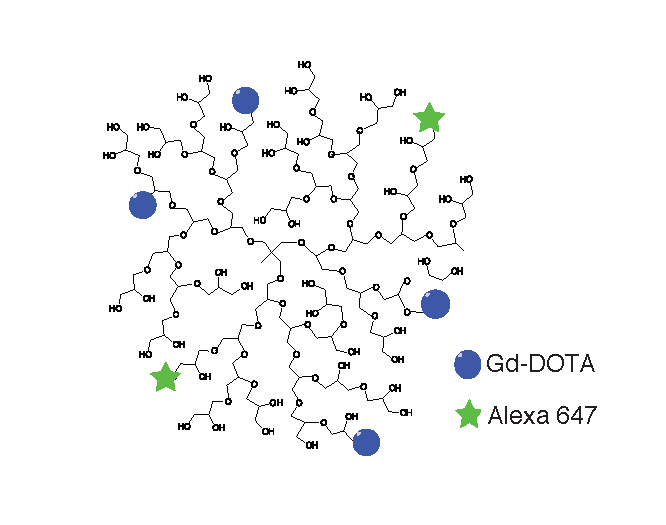
\includegraphics[width=\textwidth]{hpg/hpg-paper1-images/hpg_fig1-hpgdf.pdf}
 \caption{\acs{HPG-GdF}. The 583  \acs{kDa} globular Hyperbranched PolyGlycerol (HPG) molecules are derivatized with p-NH$_2$-benzyl-DOTA (Macrocyclics) at 20 $\mu$g Gd per mg HPG (approximately 300 chelates per molecule) and tagged with Alexa Fluor 647 dye, as previously described~\cite{Saatchi:2012hc}.}
 \label{hpgpaper1:fig1}
 \end{center}
\end{figure}

\subsection{MRI acquisition}
All MRI experiments were performed at the UBC MRI Research Centre on a 7T Bruker BioSpec 70/30 scanner at room temperature with a combination of volume (transmit)/surface (receive) coil.
Each imaging session began with axial \acs{RARE} T$_2$-weighted images for morphological reference and precise alignment of imaging plane (RARE factor 8, effective T$_E$ = 42.98 ms, T$_R$ = 4250ms, FA = 178$^{\circ}$).
In subsequent imaging sessions, slice location and orientation were adjusted to match previous sessions.

In the first scanning session, T$_1$ and flip angle maps were acquired prior to the \acs{DCE-MRI} experiment, followed by another T$_1$ measurement.
T$_1$ measurements and flip angle mapping were performed using a multi-slice FLASH variable flip angle experiment (FLASH T$_R$/T$_E$ = 500/2.75 ms, FA = 10-200$^{\circ}$ in increments of 10$^{\circ}$, and 215$^{\circ}$).
%20$^{\circ}$, 30$^{\circ}$, 40$^{\circ}$, 50$^{\circ}$, 60$^{\circ}$, 70$^{\circ}$, 80$^{\circ}$, 90$^{\circ}$, 100$^{\circ}$, 110$^{\circ}$, 120$^{\circ}$, 130$^{\circ}$, 140$^{\circ}$, 150$^{\circ}$, 160$^{\circ}$, 170$^{\circ}$, 180$^{\circ}$, 190$^{\circ}$, 200$^{\circ}$, 215$^{\circ}$).
Data were fit simultaneously for T$_1$ and the B$_1$ scaling factor map.
\acs{DCE-MRI} data was collected at 2.24~s time resolution (FLASH; T$_R$/T$_E$~=~35/2.75 ms; FA~=~40; NR~=~1200).
T$_1$ and \acs{DCE-MRI} experiments all had identical geometry (matrix = 128$\times$64; three slices; voxel size$=0.33\times 0.297\times 1.5$ mm$^3$; 2.5~mm slice separation).
A follow-up T$_1$ measurement was performed (FLASH; T$_R$/T$_E$ = 35/2.75; FA = 10$^{\circ}$, 20$^{\circ}$, 30$^{\circ}$, 40$^{\circ}$, 50$^{\circ}$, 60$^{\circ}$, 80$^{\circ}$, 100$^{\circ}$, 120$^{\circ}$) and the B$_1$ scaling factor map from the baseline acquisition was used to determine post-contrast T$_1$ (assuming that B$_1$ scaling does not change due to contrast injection).
Difference maps of relaxation rates $\Delta$R$_1=1/$T$_1$(post-contrast) - 1/T$_1$(precontrast) were constructed for a measure of contrast agent concentration.
Animals received two \acs{DCE-MRI} scans 24--48h apart, with Gadovist administered and scanned at the first session and \acs{HPG-GdF} administered and scanned at the subsequent session with tumours collected for histological processing at about 60-min post administration of their \acs{HPG-GdF}.
For qualitative assessment of contrast agent distribution  T$_1$-weighted \acs{RARE} images (RARE factor 4, effective T$_E$ = 7.5 ms, T$_R$ = 1300 ms, FA = 180$^{\circ}$) were acquired after contrast agent administration.

\begin{figure}[htbp]
 %\begin{center}
 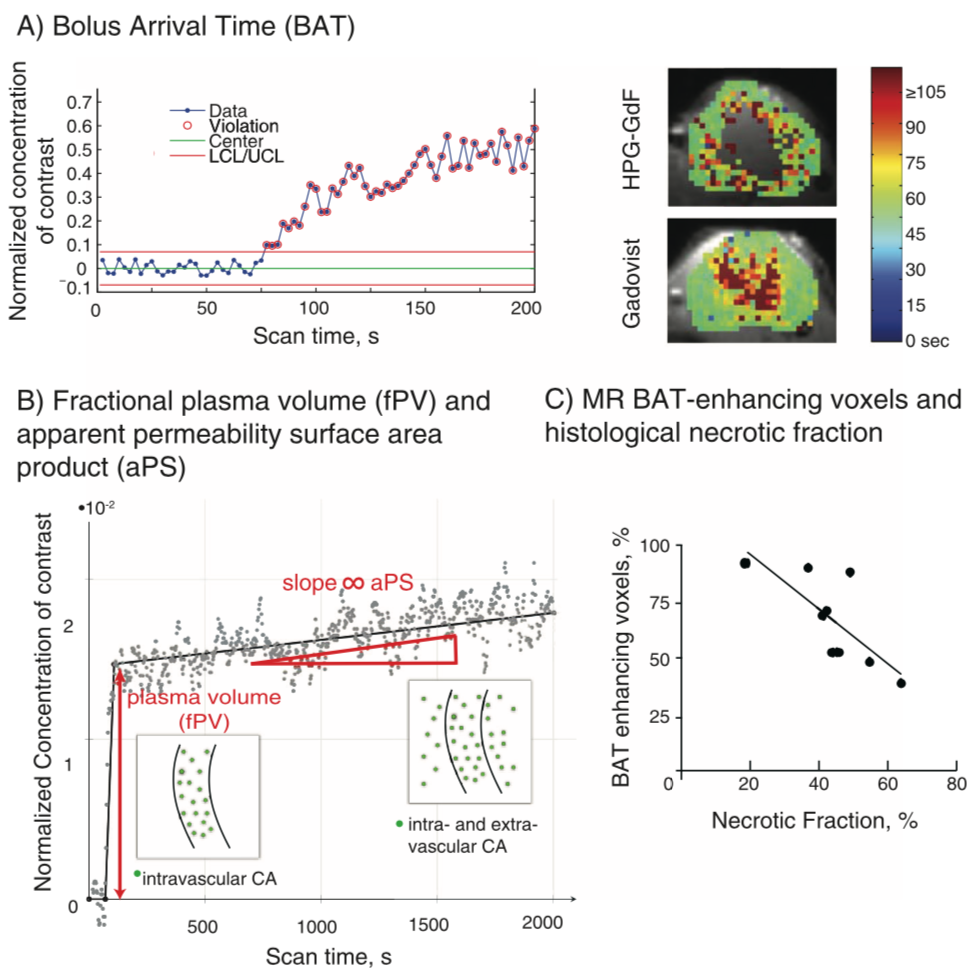
\includegraphics[width=0.9\textwidth]{hpg/hpg-paper1-images/hpg_fig2-bat.png}
 \caption{MR-derived parameters to measure vascular function using \acs{HPG-GdF}: bolus arrival time (\acs{BAT}), fractional plasma volume (\acs{fPV}) and apparent permeability-surface area product (\acs{aPS}). 
 (A) Example of how the control theory procedure was applied to determine \acs{BAT} on a sample enhancement curve showing change in concentration of \acs{CA} as a function of scan time. 
 The green line is the central line while the red lines indicate the upper and lower control limits (LCL and UCL).
 %The first violation (circle) is identified by Rule (1) at Frame 31, corresponding to a \acs{BAT} of t = 77.5 s. The centre (mean) and upper (UCL) and lower (LCL) control limits ($\pm$3 SDs) are drawn for reference. 
 (B) \acs{HPG-GdF} enhancement curve from which the \acs{fPV} is derived as the concentration at the start relative to the plasma concentration. The \acs{aPS} is the slope of the enhancement after the bolus arrival. 
 The concentration curves are shown as ratio of tissue concentration to blood peak concentration (24~$\mu$M).
 Insets within the plots are schematics of our interpretation of the situation at particular time-points and are not measured values.
 (C) The fraction of MR-measured \acs{HPG-GdF} \acs{BAT}-enhancing voxels has a negative association with the proportion of necrotic tissue determined in histological sections.}
 \label{hpgpaper1:fig2}
 %\end{center}
\end{figure}

\subsection{MRI data analysis}
\label{hpg_paper1_mrianalysis}
Regions of interest (ROIs) were drawn on T$_2$-weighted \acs{RARE} images to outline the tumour using ImageJ (NIH), and all other MR analysis was performed using MATLAB (MathWorks, R2009a) and Python.
T$_1$ and flip-angle maps were calculated from variable flip-angle data with a slice-profile correction based on simulations described by Parker et al.~\cite{Parker:2001wj}.
The same method was extended to provide time-dependent T$_1$ and concentration-time in DCE data series.
Areas under the curves (AUCs) were numerically integrated starting from the bolus arrival time, or, for tumour-averaged AUC, starting from the common injection time point and extended to the indicated time points (1 and 37 min).
Bolus arrival time (BAT) is the time when detectable signal enhancement begins for a voxel (Fig.~\ref{hpgpaper1:fig2}(A)) due to contrast agent arrival.
\acs{BAT} maps from \acs{HPG-GdF} and Gadovist obtained from the same HT29 xenograft imaged 24h apart show that \acs{HPG-GdF} is slower to arrive; both \acs{CA}s arrive most quickly at the tumour margins (Fig.~\ref{hpgpaper1:fig2}(A)). 
Based on the control-chart decision criterion and the Western Electric decision rules from MATLAB’s statistical toolbox~\cite{Shewhart:1931tq}, voxel enhancement was detected as a positive change from baseline signal for three consecutive timepoints (frames) (i) in the same direction, (ii) starting 5 s before the time of injection or later and (iii) for at least 10\% of all timepoints following initial change of signal away from baseline.
Therefore, voxels with a finite \acs{BAT} and for which at least 10\% of the following intensities were classified as enhancing by the \acs{BAT} criteria were called enhancing voxels, whereas all other voxels were labeled as non-enhancing.

A former lab member developed a set of criteria based on control theory as part of their masters thesis~\cite{McPhee:2012eu}.
A change from baseline was determined to have occurred when any one of the following inclusion criteria were met:

\begin{enumerate}
	\item any point fell outside of 3 SDs from the average baseline concentration, or
	\item two of three consecutive points fell outside of the 2 SD limit on the same side of the mean, or
	\item four of five consecutive points fell outside of the 1 SD line, on the same side of the centre line, or
	\item eight consecutive points all fell on one side of the centre line.
\end{enumerate}

In the illustrated example (Fig.~\ref{hpgpaper1:fig2}(A)), a change from the mean was identified at Frame 31 and the two following scans by Rule (1); therefore, the \acs{BAT} point was selected to be the 30$^{th}$ data point (t=67.2s).
The centre line (mean of baseline) and upper and lower control limits ($\pm$3 SDs) are drawn for reference.

\subsubsection{Pharmacokinetic modeling of DCE-MRI data}

\textit{Gadovist}: The extended Tofts model was used and three parameters resulted: \acs{K$^{trans}$}, \acs{$v_e$}, and \acs{$v_p$}~\cite{Sourbron:2011ce}.
The arterial input function (AIF) for this model was determined previously by our laboratory using a projection-based method~\cite{Moroz:2013ee} and is a four-mouse population average.

\acs{HPG-GdF} A two-parameter linear model was applied~\cite{Pathak:2005gu}.
Two parameters were used to characterize the \acs{MCA} time curves: (1) the rapid increase at the time of injection (related to the \acs{fPV}) and (2) the slope of the later enhancement (\acs{aPS}) (Fig.~\ref{hpgpaper1:fig2}(B)).
The relative plasma volume could be determined from the ratio of concentrations in the voxel of interest to the concentration in whole blood in the seconds after injection, since extra-vascular spread of the agent was negligible at this time.
The slope of the concentration time curve following contrast arrival is proportional to the permeability-surface area product (\acs{PS}) when the assumption of a permeability-limited environment is valid.
However, in the highly variable tumour microenvironment, extravasation of contrast agent may deplete the intra-vascular concentration appreciably in conditions of high permeability, which would increase the relative contribution of perfusion to the composite measure of \acs{PS}.
To stress that the interpretation of this slope value depends on the assumption of a permeability-limited environment, we term the slope the apparent permeability-surface area product (\acs{aPS})~\cite{DaldrupLink:2004gy,Dafni:2002kb}.

\subsection{Histology}

Cryosections of 10 $\mu$m were obtained along the plane perpendicular to the fiducial marker at depths corresponding to MR imaged slices.
Sections were imaged for DiOC7(3) and \acs{HPG-GdF} native fluorescence and fixed in acetone-methanol for 10min prior to staining and re-imaging for \acs{CD31} and Hoechst 3342, labeling vascular endothelium and cell nuclei, respectively.
Sections were imaged as previously described~\cite{Kyle:2007ch} using a system of tiling adjacent microscope fields of view such that images of entire tumour cryosections were captured at a resolution of 1.5 $\mu$m/pixel.
Using both fiducial and anatomical landmarks, histological sections were chosen to match the MR slices.
Using ImageJ~\cite{Collins:2007jr} and user-supplied algorithms, digital images were superimposed and manually cropped to tumour tissue boundaries; staining artifacts and necrosis were also removed for some analyses.
Positive fluorescence for \acs{CD31} and DiOC7(3) images was obtained by applying a threshold, with neighbouring positive pixels grouped as ``objects''.
The average distance of tissue to the nearest vascular object was reported as a repeatable measure of vascular density.
Perfused vessel fraction (PF) was calculated as the proportion of \acs{CD31}-positive objects that had at least 20\% overlap with positive DiOC7(3) or \acs{HPG-GdF} pixels on the overlaid image.
Data for individual tumours were displayed as mean $\pm$ SEM values.
HPG-GdF extravasation was assessed by its distance from blood vessels: pixels from the \acs{HPG-GdF} fluorescence image were sorted according to their distance from vascular objects and the average \acs{HPG-GdF} fluorescence intensity was reported.

\section{Results}

\subsection{HPG-GdF accumulates in tumour tissue in the extravascular space but does not distribute far from vasculature}

Averaged data from whole HT29 tumour xenograft images obtained using MRI and histology showed accumulation of \acs{HPG-GdF} over time (Fig.~\ref{hpgpaper1:fig3}(A)), as previously described~\cite{Saatchi:2012hc}.
\acs{HPG-GdF} fluorescence was detectable within or very near to \acs{CD31}-labeled tumour vessels as early as 2-min following contrast agent injection (Fig.~\ref{hpgpaper1:fig3}(B), (C)).
More \acs{HPG-GdF} fluorescence accumulated in histological tumour sections over time, but very little agent was observed at distances farther than 40 $\mu$m from the vasculature, even at 7 and 15 days (Fig.~\ref{hpgpaper1:fig3}(B), (C)).
By 60 min, there was extravascular accumulation of \acs{HPG-GdF} around some vessels, but considerable inter-vessel heterogeneity was observed.
Some vessels showed no \acs{HPG-GdF} fluorescence (Fig.~\ref{hpgpaper1:fig3}(C)).
Fig.~\ref{hpgpaper1:fig3}(C) also shows that \acs{HPG-GdF} accumulates over several days but does so heterogeneously, and does not distribute through tumour tissue even after prolonged exposures.

\begin{figure}[htbp]
% \begin{center}
 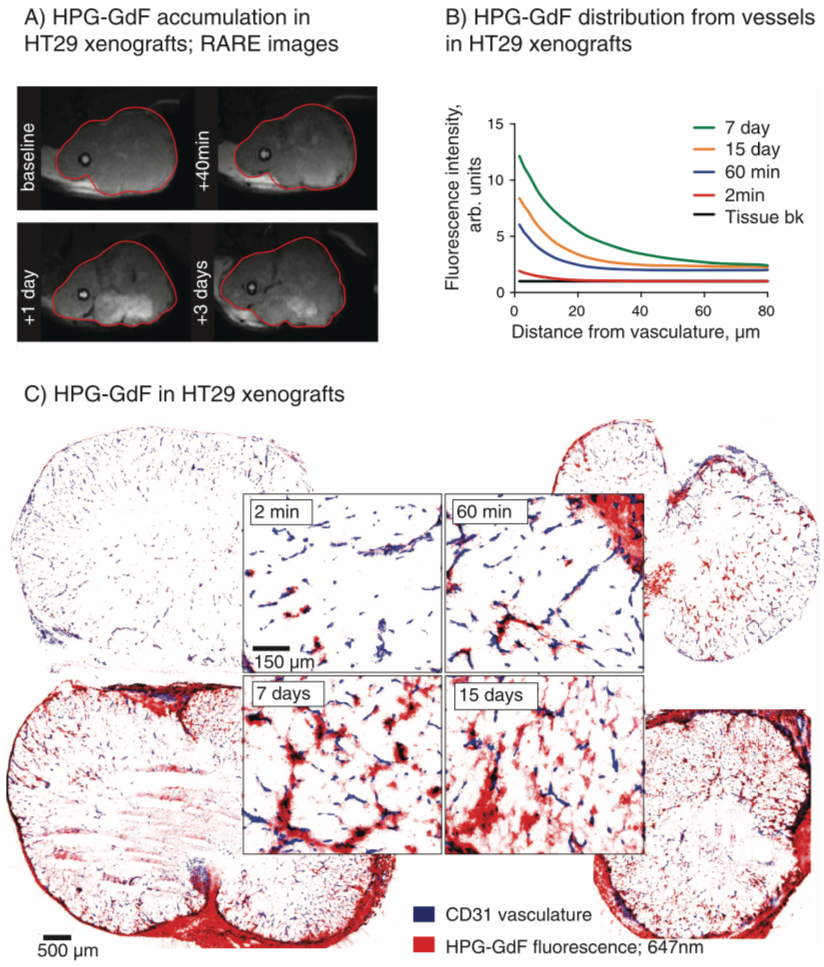
\includegraphics[width=0.9\textwidth]{hpg/hpg-paper1-images/hpg_fig3-hpgdistribution.png}
 \caption{(A) T$_1$-weighted \acs{RARE} images show signal enhancement at 40-min that increases with longer exposures (tumours outlined in red). (B) Quantitative histology shows \acs{HPG-GdF} extravasation and distribution gradually increasing with time (2-min to 7 days). (C) Whole tumour maps of \acs{HPG-GdF} (red) and vasculature (blue) show that at early (2 min) timepoints \acs{HPG-GdF} is primarily overlapped with vasculature, but by 60-min there is substantial heterogeneity, where some vessels have greater amounts of perivascular \acs{HPG-GdF} than others.}
 \label{hpgpaper1:fig3}
% \end{center}
\end{figure}

\subsection{Bolus arrival time (BAT) for \acs{HPG-GdF} as a screen for viable tissue}

Maps of \acs{BAT} overlaid on T$_1$-RARE images for both Gadovist and \acs{HPG-GdF} are shown in Fig.~\ref{hpgpaper1:fig4}, rows 1 and 2.
A pattern of faster contrast enhancement at the tumour margins was consistent for both contrast agents.
While Gadovist eventually distributes to all the tissue, many voxels fail to enhance with \acs{HPG-GdF} within the 37-min imaging period.
Comparison of \acs{BAT}-enhancing voxels with a histological image delineating viable versus necrotic tissue (Fig.~\ref{hpgpaper1:fig4}, Rows 2 and 3) shows that the non-enhancing voxels consistently corresponded to large areas of tumour necrosis.
A negative association was seen between the histological necrosis fraction and the fraction of enhancing voxels for \acs{HPG-GdF} (Fig.~\ref{hpgpaper1:fig2}(C)).
For subsequent analysis of vascular function, only voxels enhancing with \acs{HPG-GdF} using the \acs{BAT} criteria were evaluated.

\begin{figure}[htbp]
 %\begin{center}
 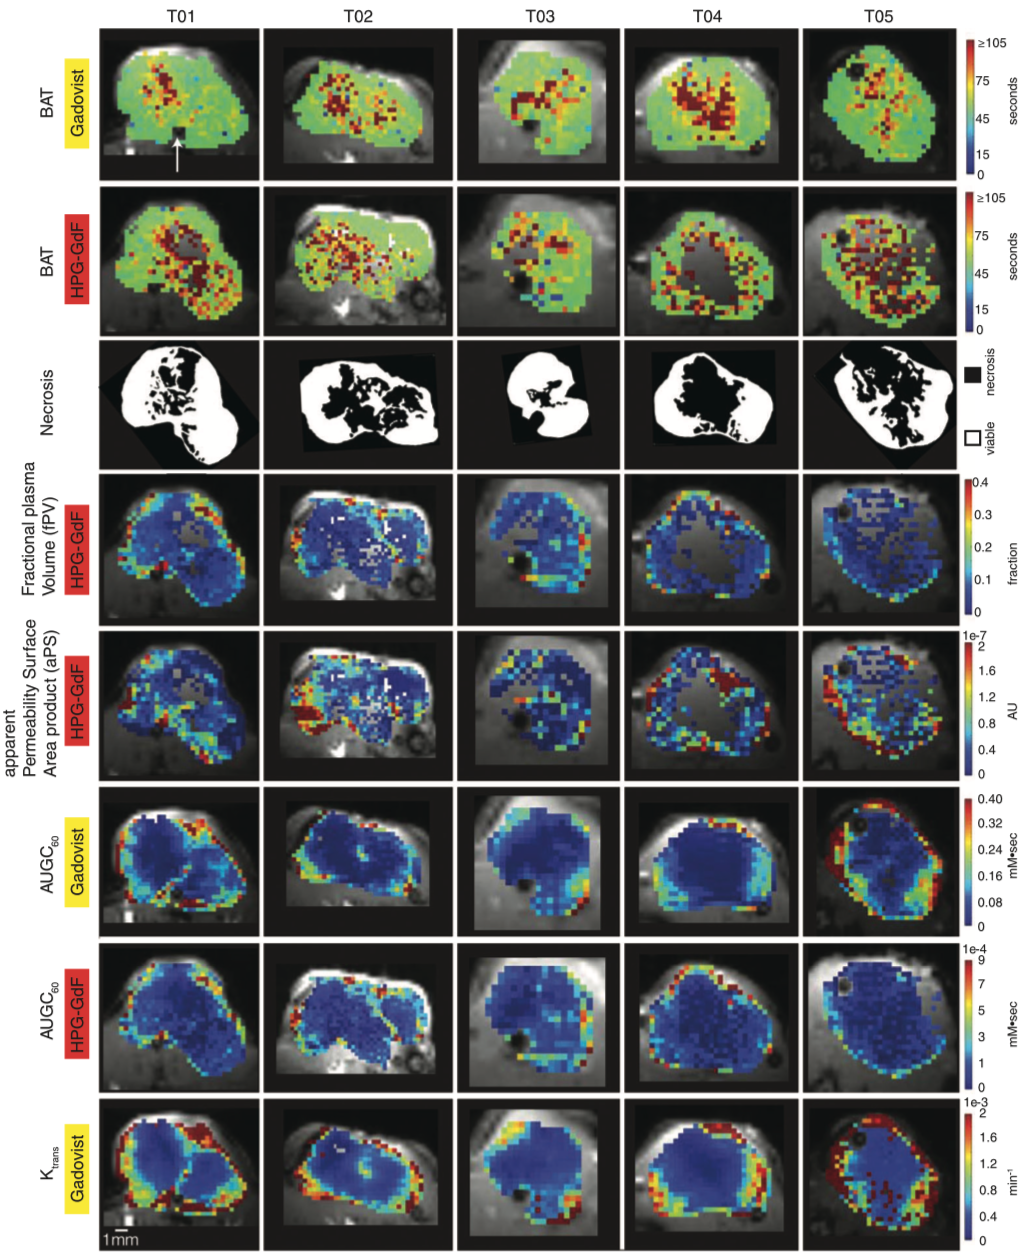
\includegraphics[width=\textwidth]{hpg/hpg-paper1-images/hpg_fig4-ht29.png}
 \caption{Individual HT29 tumour (T01-05) slice maps are presented for parameters derived using Gadovist (\acs{BAT}, \acs{AUGC$_{60}$}, \acs{K$^{trans}$}), \acs{HPG-GdF} (\acs{BAT}, \acs{fPV}, \acs{aPS}, \acs{AUGC$_{60}$}) and histological imaging of necrosis.}
 \label{hpgpaper1:fig4}
 %\end{center}
\end{figure}

\subsection{Fractional plasma volume (\acs{fPV}) and apparent permeability-surface area product (\acs{aPS}) as measures of vascular function}

\acs{HPG-GdF}-enhancing voxels were further characterized for their plasma volume (\acs{fPV}) by calculating the magnitude of the rapid signal increase after injection and for their extravascular accumulation (apparent permeability-surface area product, \acs{aPS}) by measuring the slope of the enhancement curve after the initial increase for the duration of the scan (0-2000 s).
The patterns of high and low \acs{fPV} and \acs{aPS} were often similar to each other, though there are notable differences.
A linear regression analysis comparing \acs{fPV} with \acs{aPS} for whole-slice averages yields an R$^2$ of 0.11, suggesting they are independent of each other.
As a detailed example, tumour HT01 has a region of high \acs{aPS} and low \acs{fPV} (Fig.~\ref{hpgpaper1:fig5}(A)), as well as a region exhibiting the opposite, with high \acs{fPV} and low \acs{aPS} (Fig.~\ref{hpgpaper1:fig5}(B)).
The corresponding histological section seemed to validate these observations, where the region with high \acs{fPV} has a greater density of \acs{CD31}-stained vessels and the region with greater \acs{aPS} has more \acs{HPG-GdF} in the extravascular compartment.
While histological data enables a detailed view of \acs{HPG-GdF} accumulation, the actual rate of extravasation may only be determined by the dynamic MR data, as illustrated by the schematic enhancement curve (Fig.~\ref{hpgpaper1:fig5}(C)).
The corresponding K$^{trans}$ map derived from Gadovist concentrations shows high values in both the high \acs{aPS} and high \acs{fPV} regions of this tumour (Fig.~\ref{hpgpaper1:fig4}, Column 1).
Therefore, both \acs{fPV} and \acs{aPS} played important roles contributing to overall tumour vascular function, had measurable intra-tumour heterogeneity and produced data that was distinct from and more informative than \acs{DCE-MRI} derived parameters for Gadovist.

\begin{figure}[htbp]
 \begin{center}
 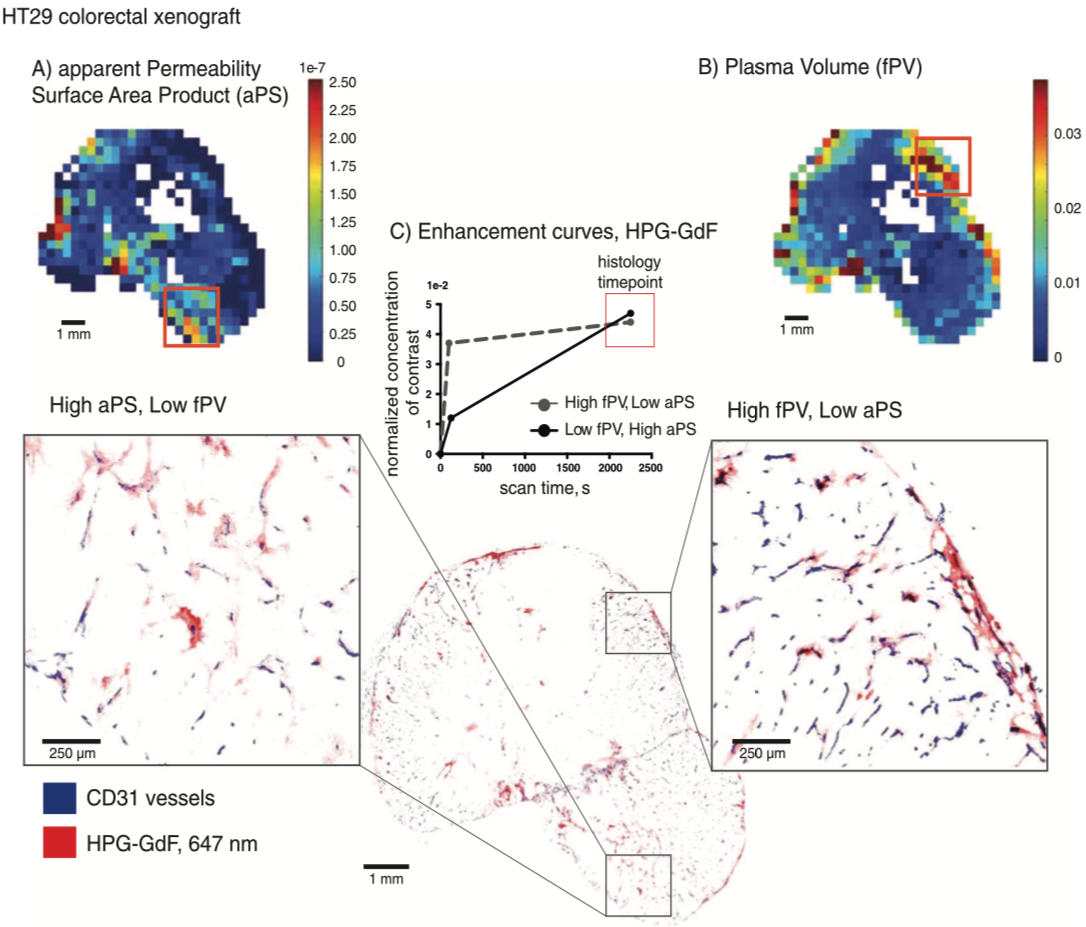
\includegraphics[width=\textwidth]{hpg/hpg-paper1-images/hpg_fig5-ht29fpv.png}
 \caption{\acs{fPV} and \acs{aPS} parameter maps for an HT29 tumour (T01) are shown with corresponding histological image depicting \acs{CD31}-stained vessels (blue) and \acs{HPG-GdF} native fluorescence (red).
 The high \acs{fPV} region has notably greater vascular density, and \acs{HPG-GdF} is clearly seen overlapping with vessels (black) or accumulating in the extravascular space.
 A region with high \acs{aPS} that does not correspond to high \acs{fPV} is magnified (A) and compared with a high \acs{fPV} region that does not correspond to high \acs{aPS} (B).}
 \label{hpgpaper1:fig5}
 \end{center}
\end{figure}

\subsection{Variable vascular function in HCT116 and HT29 human colorectal xenografts}

HPG-GdF accumulated to a greater degree in HT29 colorectal xenografts relative to HCT116, and this was seen at all distances from vessels (Fig.~\ref{hpgpaper1:fig6}(A)).
HCT116 and HT29 colorectal xenografts grow at similar rates in mouse models but exhibit distinct vascular function parameters (data summarized in Table~\ref{hpgpaper:table1}).
Overall, HT29 tumours possessed a greater density of vessels (\acs{CD31} average distance was $82.3\pm 3.0~\mu$m for HCT116 and $40.5\pm 1.5~\mu$m for HT29, $p<0.05$).
However many vessels were unlabelled for the fluorescent dye (carbocyanine) used as a histological perfusion marker; the density of perfused vessels was similar between the two xenograft models (\acs{CD31} vessels labeled for carbocyanine, PF, was $47.8\pm 5.4$\% for HCT116 and $36.0\pm 2.1$\% for HT29, $p>0.05$).
The density of vessels labeled for \acs{HPG-GdF} fluorescence was much greater in HT29 tumours (HPG-GdF+ve \acs{CD31}, average distance was $172\pm 10~\mu$m for HCT116 and $88.9\pm 6.3~\mu$m; $p < 0.05$).
In addition to a greater density of \acs{HPG-GdF}-positive vessels, the high \acs{MW} contrast agent was able to accumulate to a greater degree in the extra-vascular space around vessels in HT29 cells.
This effect can be seen in the histological images of the compared tumour models collected 60-min post \acs{HPG-GdF} administration (Fig.~\ref{hpgpaper1:fig6}(B)).

\begin{table}[htbp]
\begin{center}
    \rowcolors{2}{gray!10}{white}
    \begin{tabular}{@{}p{3.2cm}clll@{}}
    \rowcolor{gray!50}
Histological Quantity & Units & HCT116 & HT29 & p-value  \\
%\hline
CD31 \newline(Average distance) & $\mu$m & 82.3$\pm$3.0    & 40.5$\pm$1.5    & 0.008 \\
Carbocyanine \acs{PF} & \%                        & 47.8$\pm$5.4    & 36.0$\pm$2.1    & 0.11    \\
Carbocyanine-positive and CD31 (Average distance)                           & $\mu$m               & 137$\pm$13      & 95.0$\pm$11.5   & 0.11    \\
\acs{HPG-GdF} \acs{PF}                        & \%                        & 19.9$\pm$2.0    & 23.4$\pm$1.2    & 0.31    \\
\acs{HPG-GdF}-positive and CD31  (Average distance) & $\mu$m               & 172$\pm$10      & 88.9$\pm$6.3    & 0.008\\
\acs{HPG-GdF} (Average intensity) & a.u. & 0.405$\pm$0.031 & 0.828$\pm$0.123 & 0.008 \\
Necrosis Fraction                                        & \%                       & 52.4$\pm$3.6    & 37.7$\pm$5.1    & 0.032 
\end{tabular}
\caption{Summary of the quantitative histological histological data for the HCT116 and HT29 tumours.}
\label{hpgpaper:table1}
\end{center}
\end{table}

\subsection{MRI analysis of \acs{HPG-GdF} in HCT116 and HT29 xenografts: \acs{BAT}, \acs{fPV} and \acs{aPS}}

Administration of neither Gadovist nor \acs{HPG-GdF} was useful in detecting the difference in vascular function between HCT116 and HT29 tumours using the initial area under the gadolinium concentration curve (\acs{AUGC$_{60}$}).
The slice-averaged means were not significantly different between tumour groups (data summarized in Tables~\ref{hpgpaper:table2} and \ref{hpgpaper:table3}).
%(\acs{AUGC$_{60}$} for Gadovist in HCT116 was $5.09\pm 0.83$~mM$\cdot$s and \acs{AUGC$_{60}$} for Gadovist in HT29 was $7.68\pm 1.66$~mM$\cdot$s, ${p>0.05}$; \acs{AUGC$_{60}$} for \acs{HPG-GdF} in HCT116 was $6.41\pm 1.71\times 10^{-3}$~mM$\cdot$s and that in HT29 was $9.62\pm 1.64\times 10^{-3}$~mM$\cdot$s, ${p>0.05}$) 
Similarity between models was also observed qualitatively in the parameter maps with \acs{AUGC$_{60}$} or K$^{trans}$ overlaid on T$_1$-RARE images shown in Figs.
\ref{hpgpaper1:fig4} and \ref{hpgpaper1:fig7}.
Both tumour models show higher \acs{AUGC$_{60}$} values in the tumour margins for both contrast agents.

\begin{table}[htbp]
    \rowcolors{2}{gray!10}{white}
\begin{tabular}{@{}lllll@{}}
    \rowcolor{gray!50}
%\toprule
Gadovist quantity  & units     & HCT116         & HT29           & p value \\ %\midrule
AUGC$_{60s}$  & mM$\cdot$s      & $5.09\pm0.83$      & $7.68\pm1.66$      & 0.31 \\
AUGC$_{37min}$ & mM$\cdot$s      & $317\pm23$         & $395\pm70$         & 0.56 \\
\acs{$v_p$}          & \% & $9.92\pm1.87\times10^{-3}$ & $9.03\pm3.27\times10^{-3}$ & 0.42    \\
\acs{$v_e$}          & \% & $0.247\pm0.024$    & $0.246\pm0.013$    & 0.77    \\
\acs{K$^{trans}$}  & min$^{-1}$     & $8.41\pm1.56\times10^{-4}$  & $1.16\pm0.039\times10^{-3}$ & $>$0.99   \\
R$^2$ (p75)    &    -       & $0.892\pm.017$     & $0.913\pm.018$     & 0.31    \\
BAT         & seconds   & $69.5\pm4.2$       & $62.7\pm2.3$       & 0.31    \\
BAT-EV      & \%         & $98.9\pm0.6$       & $99.2\pm0.5$       & 0.63    \\ 
\end{tabular}
\caption{Summary of MRI parameters derived from pharmacokinetic modeling of the Gadovist contrast agent for both the HCT116 and HT29 tumours.}
\label{hpgpaper:table2}
\end{table}

% Please add the following required packages to your document preamble:
% \usepackage{booktabs}
\begin{table}[htbp]
    \rowcolors{2}{gray!10}{white}
\begin{tabular}{@{}lllll@{}}
    \rowcolor{gray!50}
%\toprule
\acs{HPG-GdF} quantity & units     & HCT116           & HT29             & p value \\%\midrule
IAUC$_{60s}$  & mM$\cdot$sec    & $6.41\pm1.71 E-03$ & $9.62\pm1.64E-03$  & 0.15   \\
AUC$_{37min}$  & mM$\cdot$sec    & $0.384\pm0.097$    & $0.532\pm0.050$    & 0.31   \\
\acs{BAT}         & seconds   & $83.3\pm5.0$       & $83.6\pm7.0$       & 0.53   \\
BAT-EV      & \%         & $52.2\pm4.8$       & $81.8\pm5.0$       & 0.016 \\
\acs{fPV}         & fraction  & $1.07\pm0.33E-02$  & $0.864\pm0.27E-02$ & 0.22   \\
\acs{aPS}         & seconds$^{-1}$ & $2.38\pm1.00E-08$  & $5.81\pm1.4E-08$   & 0.06  %\\ \bottomrule
\end{tabular}
\caption{Summary of MRI parameters derived from applying a linear model to the \acs{HPG-GdF} contrast kinetics for both the HCT116 and HT29 tumours.}
\label{hpgpaper:table3}
\end{table}

\begin{figure}[htbp]
 \begin{center}
 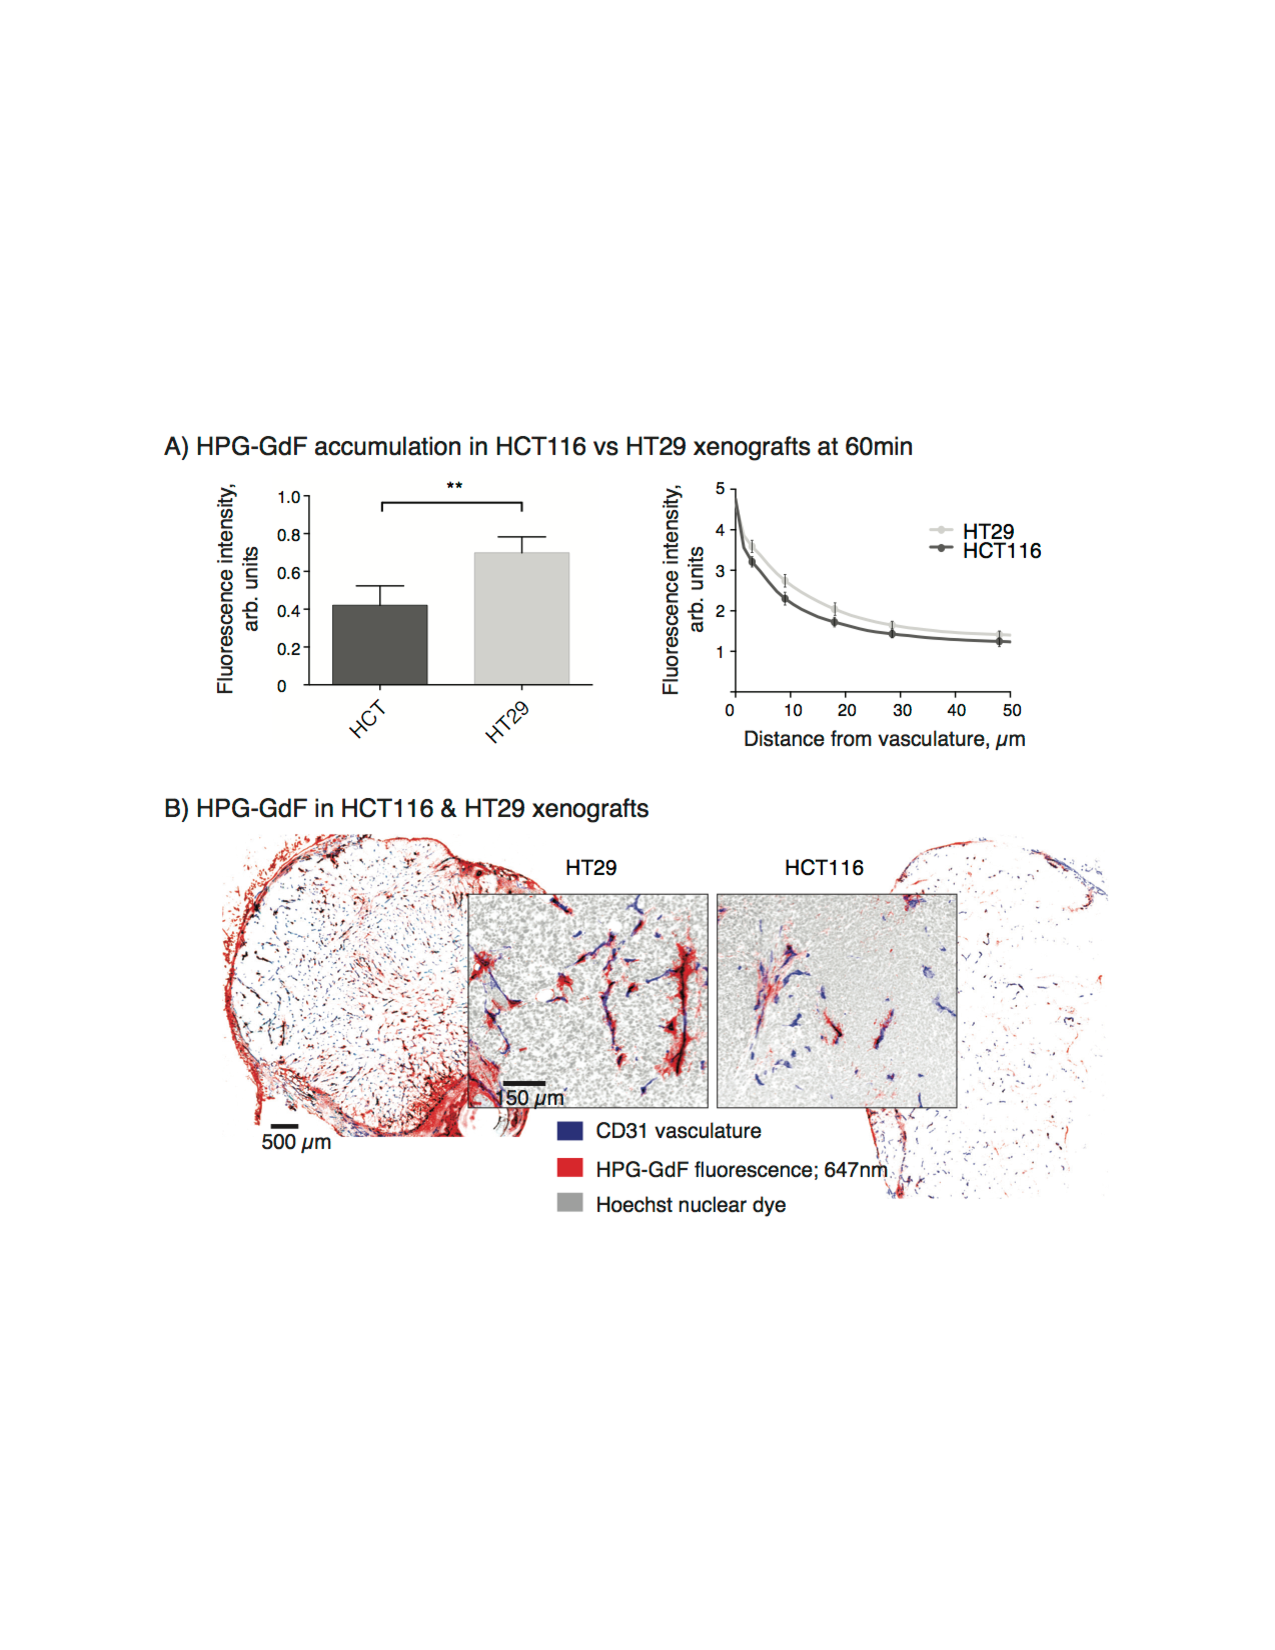
\includegraphics[width=\textwidth]{hpg/hpg-paper1-images/hpg_fig6-accumulation.pdf}
 \caption{HPG-GdF distribution in HCT116 and HT29 colorectal tumour xenografts at 60-min: histological analysis.
 (A) The whole-slice average fluorescence intensity shows that \acs{HPG-GdF} accumulates to a greater degree and distributes further away from vasculature in HT29 tumours.
 (B) Sample images show \acs{HPG-GdF} (red) overlaid on \acs{CD31} (blue); insets also display nuclear density (grey).
 A greater degree of \acs{HPG-GdF} accumulation can easily be appreciated in the HT29 tumours.}
 \label{hpgpaper1:fig6}
 \end{center}
\end{figure}

However, an MR-measured difference between HCT116 and HT29 vascular function was seen with the \acs{BAT} data for \acs{HPG-GdF}.
The fraction of enhancing voxels was significantly lower in the HCT116 relative to the HT29 tumours (BAT-enhancing voxels for \acs{HPG-GdF} in HCT116 was $52.2\pm 4.8$\% and was $81.8\pm 5.0$\% in HT29, $p=0.016$ ) (Table~\ref{hpgpaper:table3}).
This corresponded to the histological data, which also shows HCT116 tumours as having a greater proportion of necrotic tissue (necrosis fraction for HCT116 was $52.4\pm 3.6$\% vs. $37.7\pm 5.1$\% in HT29, $p=0.03$).
Of the \acs{HPG-GdF} \acs{BAT}-enhancing voxels, the averaged \acs{fPV} and \acs{aPS} parameters were also determined (Table~\ref{hpgpaper:table3}), and no difference was seen with the plasma volume between tumour models (fractional \acs{fPV} for HCT116 is $2.67\pm 0.33\times10^{-4}$ and is $2.16\pm 0.27 \times10^{-4}$ for HT29).
\acs{aPS} of \acs{HPG-GdF} was the only MR-derived biomarker able to detect the significant difference in vascular function between these two tumour models.
Complete data sets for HCT116 tumours are shown in Fig.~\ref{hpgpaper1:fig7}.

\section{Discussion}

The use of \acs{MCA}s for imaging and describing tumour vascular function is a widely pursued area of research.
Many studies have investigated a range of sizes, where smaller molecules extravasate and distribute through tissue too quickly to be considered as sensitive blood pool agents, and larger molecules often accumulate too slowly for adequate signal detection~\cite{Kyle:2007ch,Tang:2013fi,Sourbron:2011ce}.
In this work we describe \acs{HPG-GdF} as an MR-visible \acs{MCA} of 583~\acs{kDa}, for which we have derived useful biomarkers that have sensitivity in measuring vascular function in preclinical studies.
The agent HPG-GdF is not intended to be used in patients directly primarily because of differences in human and tumour xenograft vessel morphology, as well as the unknown safety, efficacy, and biocomaptibility considerations of the agent in humans.
However, despite this \acs{HPG-GdF} may be very useful in developing drugs and understanding the distribution of existing drugs in preclinical experiments.

While the signal-to-noise ratio (\acs{SNR}) from \acs{HPG-GdF} concentration-time curves is not adequate to fit a complex pharmacokinetic model to determine parameters such as \acs{$v_p$}, \acs{$v_e$} and \acs{K$^{trans}$}, enhancement was measurable in most tumour voxels.
The number of Gd chelates on the \acs{HPG-GdF} is approximately 300 per carrier molecule, which is high relative to many albumin chelates, the most common \acs{MCA} in preclinical use, which typically have about 20 chelates per carrier~\cite{Ogan:1987tg}.
In addition to a greater number of Gd per carrier, the \acs{HPG-GdF} accumulates in the perivascular space and fails to distribute more than a few micrometers from most vessels within a short DCE imaging timeframe (Fig.~\ref{hpgpaper1:fig3}).
This accumulation could provide a greater concentration for detection of a local, permeable tumour vessel and avoids the risk of conflating this with the distribution and accumulation elsewhere in tumours.
These attributes of \acs{HPG-GdF} may make it more sensitive and more specific than a smaller \acs{MCA} such as albumin-Gd-DTPA.
A minimum DCE imaging time from the presented data would appear to be about 15~min for the analyses described, which is longer than the suggested 5-min ideal for practical clinical utility~\cite{Turetschek:2004bw}.
It is possible that greater signal could also be obtained by decreasing the time resolution from the 2.24 s used in these studies, since \acs{HPG-GdF} remains largely intravascular.

\acs{HPG-GdF} contains the Gd-\acs{DOTA} complex, which is thermodynamically highly stable and kinetically inert.
The dissociation constant for Gd-\acs{DOTA} ($\log K = 24.7$) is much higher than those for Ca-\acs{DOTA} ($\log K = 17.23$) or Mg-\acs{DOTA} ($\log K = 11.92$), hence neither Ca nor Mg can transmetallate Gd from the Gd-\acs{DOTA} complex~\cite{Baranyai:2005ta}.
Biodegradation of \acs{HPG-GdF} is therefore likely minimal, occurring through enzymatic attack of the end group, similar to that seen for polyethylene glycol~\cite{Kawai:2002fc}.
However, the long half-life and relatively slow excretion of HPGs through the reticuloendothelial system of the liver suggest that the potential for toxicity should be investigated and monitored.
A biodegradable version of HPG has recently been synthesized and might circumvent these potential concerns, and will be a focus in future \acs{DCE-MRI} studies investigating the use of HPGs as MR-visible \acs{MCA}s~\cite{Shenoi:2013id}.

Limited distribution through the interstitium is also most probably the result of its significant size.
We have observed \acs{HPG-GdF} to be much more restricted in its distribution than is suggested by the diffusion coefficients (D$_{HPG}$ = 3.7$\times$10$^{-7}$ cm$^2$ s$^{-1}$ and D$_{Gadovist}$ = 3.6$\times$10$^{-6}$ cm$^2$ s$^{-1}$), as the larger agent reaches only 10-15 $\mu$m away from vessels within an hour whereas Gadovist reaches all areas of a tumour.
\acs{HPG-GdF} molecules experience greater obstacles to their movement through the heterogeneous tumour microenvironment due to their size, but also possibly due to steric hindrances, non-specific binding or sequestration~\cite{Minchinton:2006gs}.

The large size of \acs{HPG-GdF} is a significant advantage.
An approximately exponential increase in sensitivity for detection of permeability has been reported with increasing MCA size (19).
If extravasation of \acs{HPG-GdF} only occurs in vessels that are permeable, and the agent does not distribute through the extravascular space to distances away from vessels, then MR-visible \acs{HPG-GdF} enhancement suggests the presence of vasculature, and accumulation of the agent over time indicates the local presence of a hyper-permeable vessel.

\begin{figure}[htbp]
 \begin{center}
 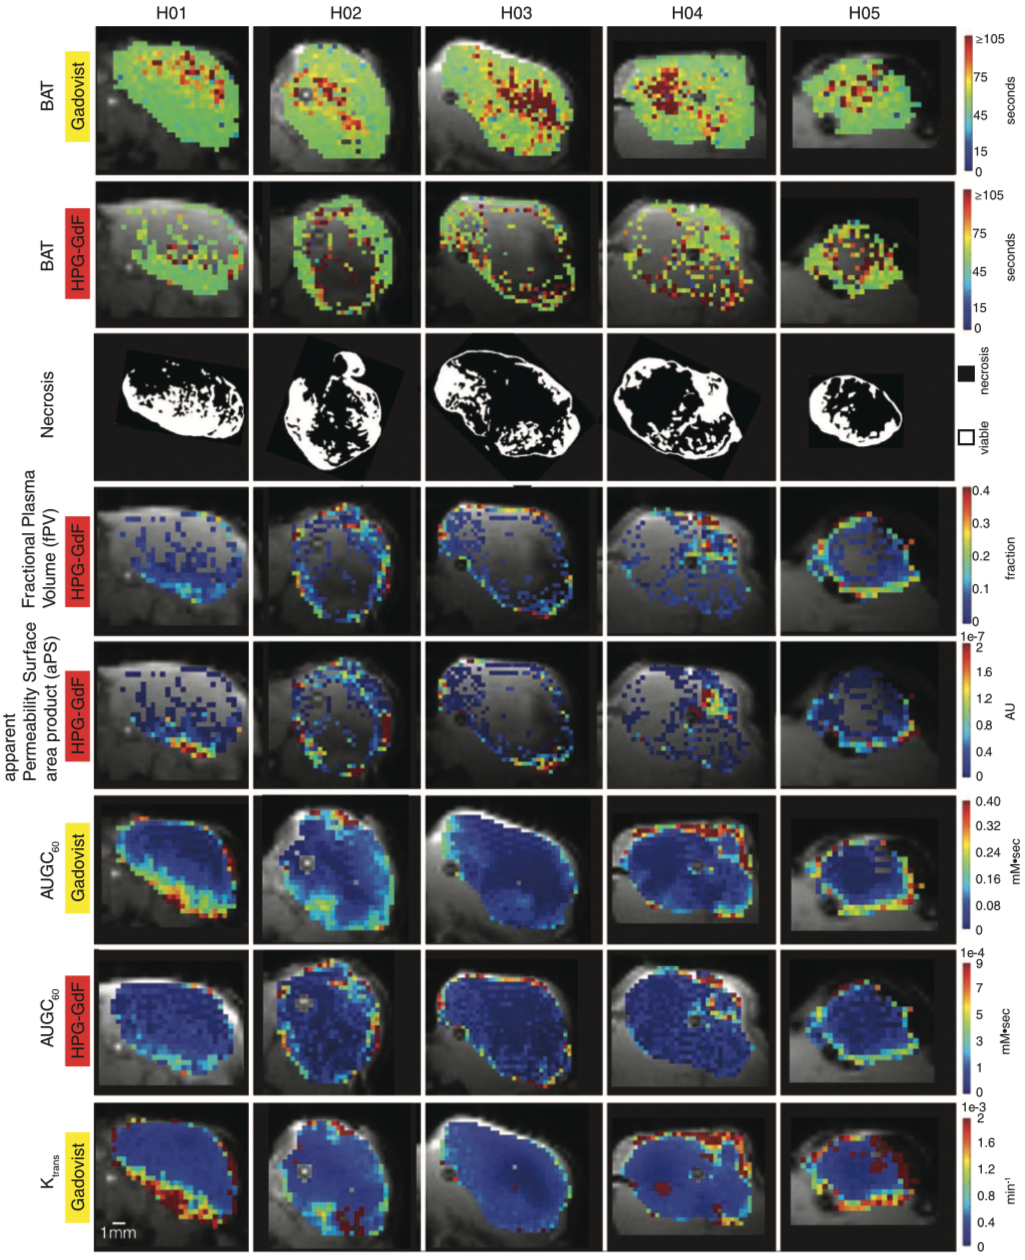
\includegraphics[width=\textwidth]{hpg/hpg-paper1-images/hpg_fig7-hct116.png}
 \caption{Vascular function in HCT116 xenografts. Whole-slice maps are presented for individual HCT116 tumours (T01-T05, vertical columns) for parameters derived from MR imaging of Gadovist (BAT, \acs{AUGC$_{60}$}, K$^{trans}$), MR imaging of \acs{HPG-GdF} (\acs{BAT}, \acs{fPV}, \acs{aPS}, \acs{AUGC$_{60}$}) and histological imaging (necrosis).}
 \label{hpgpaper1:fig7}
 \end{center}
\end{figure}

A typical enhancement curve for \acs{HPG-GdF} is shown in Fig.~\ref{hpgpaper1:fig2}.
The size of the initial step-like enhancement is interpreted as the \acs{fPV}, and the slope of signal change for the remaining enhancement is reported as the \acs{aPS}, reflecting the extravascular accumulation of \acs{HPG-GdF} (Fig.~\ref{hpgpaper1:fig2}).
These parameters are not correlated with each other, with either value potentially significantly higher or lower than the other in the same voxels (Fig.~\ref{hpgpaper1:fig5}).
A pattern of faster enhancement at the tumour margins is consistent for both contrast agents, and, while Gadovist eventually arrives in all the tissue, including regions of necrosis, many voxels that correspond to necrotic regions fail to enhance with \acs{HPG-GdF} within the 37-min imaging session.
We found that \acs{HPG-GdF} \acs{BAT}-enhancing voxels correspond to areas without necrosis: see Figs.~\ref{hpgpaper1:fig4} and ~\ref{hpgpaper1:fig7} for parameter maps of all \acs{BAT}-enhancing voxels compared with histologically validated necrotic regions.
Therefore, we identified perfused regions of tumour tissue for further vascular function analysis using the straightforward approach of selecting voxels that had positive \acs{BAT}s for their \acs{HPG-GdF} enhancement curves.
Selection of viable tissue and the exclusion of necrotic tissue is a desirable approach for controlling for inter-tumour heterogeneity, since MRI data is most often described as a whole-tumour average.
In the event that different tumours possess variable necrotic burdens, or if the necrotic fraction increases over time with treatment, selective analysis of viable tissue can control for this variability.

Qualitative comparisons of well-matched, whole-slice images from multiple modalities emphasize the utility of screening for \acs{BAT}-enhancing voxels to select for perfused and viable tissues.
Without this information, analysis may be restricted to regions of tissues at the tumour margins where hot spots of vascularization are observed histologically, and tissue is assumed to be viable in the MR image~\cite{Pathak:2005gu,Li:2005gw}.
In the colorectal xenografts examined here, the amount of necrosis varied considerably, and while necrosis is typically located more in the core than the tumour margins, there is substantial inter-tumour heterogeneity with respect to the amount and location of necrosis.
Notably, while the values for \acs{K$^{trans}$} using Gadovist are on average higher around the entire tumour rim, the \acs{fPV} and \acs{aPS} values are more heterogeneously arranged around the rim and within the interior of the tumour.
Our more comprehensive approach, validated by observations of viable tissue and perfused vessels within tumour interiors in histological sections, is a significant improvement over selectively assessing limited regions or hotspots for histological or MR quantitative analysis.

Traditional DCE-derived parameters such as \acs{AUC} and \acs{K$^{trans}$} are composite measures influenced to varying degrees by vascular surface area, permeability and blood flow.
Our histological data supports a significant range in the propensity for \acs{HPG-GdF} to extravasate, suggesting that assumptions of perfusion or permeability-limited conditions are not applicable to all areas of the tumour microenvironment.
Hence, we cannot conclude that \acs{aPS} is exclusively proportional to permeability-surface area (PS) in the whole microenvironment.
For example, although the amount of \acs{HPG-GdF} leaking into the extravascular space is dependent on the vessel being permeable to large molecules, the amount of accumulation, and therefore the amount of signal enhancement, may still be impacted by the concentration of contrast agent within the vessel.
Longitudinal gradients can occur locally in permeable vessels as the contrast agent leaks out, despite plasma concentrations remaining consistent in overall systemic circulation~\cite{Erickson:2003wt,Dewhirst:1999jh}.
Thus, the \acs{aPS} is a measure of vascular function that has contributions from permeability as well as, when permeability is very high, perfusion.
These limitations in the physiological interpretation of \acs{aPS} are similar to those that apply to K$^{trans}$ and \acs{AUC} for all contrast-enhanced modelling.

Parameters that are based on the amount and proportion of contrast agent enhancement are dependent on fewer assumptions than are pharmacokinetic model-derived parameters such as K$^{trans}$.
Biophysical signals are dependent on the many variables necessarily involved in obtaining MR images, such as the scanner, imaging sequence, RF coil and analysis techniques.
Interpreting magnitudes of change in highly variable tumours may be more reliable than assuming invariable pharmacokinetic attributes or unchanging tumour microenvironments, and may make simplified biomarkers such as \acs{fPV} and \acs{aPS} more applicable to clinical studies conducted across multiple centres~\cite{OConnor:2012ie}.

\section{Conclusion}

HPG-GdF is a largely intravascular MCA that selectively extravasates from hyperpermeable tumour vessels, accumulating in the perivascular regions without distributing through the tumour interstitium.
The high concentration of Gd chelates per carrier molecule in combination with its excellent solubility makes \acs{HPG-GdF} detection possible despite the relatively low plasma fraction within tumours.
By carefully comparing the vessel parameters of small and large molecule contrast agents in the same tumour, as well as comprehensively assessing the location of MCA within the tumour relative to vasculature and necrosis, we conclude that \acs{BAT}, \acs{fPV} and \acs{aPS} biomarkers derived from \acs{HPG-GdF} enhancement provide a sensitive and specific approach to measuring tumour vascular function.
When assessing the significant differences in vascular function of two tumour models (HCT116 and HT29), \acs{HPG-GdF} was useful in detecting a difference (\acs{aPS}) while no change was measured with parameters derived from Gadovist.
Thus we conclude that \acs{HPG-GdF} and these analysis techniques are appropriate in the evaluation of tumour angiogenesis and response to treatment for preclinical research.

\endinput
